\subsection{Explain the origin of the molecular potential within the Born-Oppenheim approximation and discuss the vibrational and rotational structure of diatomic molecules.}


Et molekyle er ikke blot stift (eng. rigid), men det kan rotere og vibrere, hvilket vi vil tage højde for nedenfor, hvilket betyder, at vi skal tage højde for atomkernens bevægelse, når vi regner Schrödingerligningen $\Hat{H}\psi = E \psi$, hvorfor vores Hamiltonoperator nu bliver
\begin{align}
    \Hat{H} &= \Hat{H}_0 + \Hat{H}' \: , \quad \text{hvor} \quad \Hat{H}_0 = \Hat{T}_e + V \: , \quad \Hat{H}' = \Hat{T}_k \: .
\end{align}
Her er $\Hat{T}_e$ elektronernes kinetiske energi, $V$ er potentialet og $\Hat{T}_k$ er kernens kinetiske energi. Her har vi benyttet, at atomets kerne har langt større masse end elektronerne, men den bevæger sig også utrolig langsomt, og af denne grund kan det antages som en god approksimation, at elektronerne vil indrette sig instantant til kernens ændringer, hvilket giver ovenstående Hamiltonoperator. Den kinetiske energi af kernen $T_k$ er så lille, at vi ser den som værende en perturbation til den kendte Hamiltonoperator for elektronernes bevægelse $\Hat{H}_0$.
Vi kender altså løsningen til Schrödingerligningen for $\Hat{H}_0$
\begin{align}
    \hat{H}_0\phi^{el}(\Vec{r}, \Vec{R}) &= E^{(0)}(\Vec{R})\phi^{el}(\Vec{r}, \Vec{R}) \: ,
\end{align}
hvor $\phi^{el}(\Vec{r},\Vec{R})$ giver en komplet og ortogonal basis.

Vi benytter os af \textsf{Born-Oppenheimerapproksimationen}\footnote{Introduceret i 1927 af Max Born og Robert Oppenheimer.}, som negligere vekselvirkningen mellem kernens og elektronernes bevægelse, igen da elektronerne instantant indretter sig kernens bevægelser. Den totale løsning kan derfor skrives som et produkt af kernens og elektronernes bølgefunktioner
\begin{align}
    \psi(\Vec{r}, \Vec{R}) &= \sum_m \chi_m(\Vec{R}) \phi_m^{el}(\Vec{r}, \Vec{R}) \: .
\end{align}

Indsættes denne bølgefunktion i Schrödingerligningen med den fuldstændige Hamiltoperator, og multipliceres fra venstre med den $n$'te elektrons bølgefunkion, så fås
\begin{align}
    \int \left[\phi_n^{el} (\Hat{H} - E) \sum_m \chi_m\phi_m^{el}\right] \, \text{d}\Vec{r} &= 0 \: .
\end{align}
Siden vi har $\Hat{H} = \Hat{H}_0 + \Hat{H}'$, så vil integralet kunne opdeles, og den kendte løsning til Schrödingerligningen med $\Hat{H}_0$ indsættes
\begin{align}
    (E_n^{(0)} - E)\chi_n 0 + \int \phi_n^{el} \Hat{H}'\sum_m \chi_m\phi_m^{el} \, \text{d}\Vec{r} &= 0 \: ,
\end{align}
hvor det ovenstående integral kan beregnes til
\begin{align}
    &\int \phi_n^{el}\sum_m \left(\Hat{H}'\chi_m\right)\phi_m^{el} \, \text{d}\Vec{r} + \int \phi_n^{el}\sum_m \chi_m\left(\Hat{H}'\phi_m^{el}\right) \, \text{d}\Vec{r} \nonumber\\
    &\qquad \qquad \qquad \qquad \qquad \quad - \hbar \int \phi_n^{el} \sum_k \frac{1}{M_k} \sum_m \frac{\partial}{\partial R_k} \phi_m^{el} \frac{\partial}{\partial R_k} \chi_m \, \text{d}\Vec{r} \nonumber\\
    =& \int \phi_n^{el}\sum_m \left(\Hat{H}'\chi_m\right)\phi_m^{el} \, \text{d}\Vec{r} + c_{nm} \: ,
\end{align}
hvor $M_k$ er kernens masse.

Vi kan altså skrive løsningen til de to dele af den totale Hamiltonoperator som to adskilte Schrödingerligninger
\begin{align}
    \Hat{H}_0 \phi^{el}(\Vec{r}, \Vec{R}) &= E_{(0)}(\Vec{R})\phi^{el}(\Vec{r}, \Vec{R}) \: , \\
    \Vec{T}_k \chi_n(\Vec{R}) + \sigma_m c_{nm} \chi_m(\Vec{R}) &= (E - E_n^{(0)}(\Vec{R}) \chi_m(\Vec{R}) \: ,
\end{align}
og benytter vi os af Born-Oppenheimerapproksimationen ($\Rightarrow c_{nm} = 0 \: \forall n,m$) fås de følgende afkoblede ligninger
\begin{align}
    \Hat{H}_0 \phi^{el}(\Vec{r}, \Vec{R}) &= E^{(0)}(\Vec{R})\phi^{el}(\Vec{r}, \Vec{R}) \: , \\
    \Vec{T}_k \chi_n(\Vec{R}) + \sigma_m c_{nm} \chi_m(\Vec{R}) &= \{E - E_n^{(0)}(\Vec{R})\} \chi_m(\Vec{R}) \: ,
\end{align}
hvilke kan løses hver for sig, da koblingsledet er blevet negligeret.
Den første ligning beskriver en elektronbølgefunktionen for et stift (eng. rigid) molekyle, hvor elektronerne er i tilstanden $n,\, L,\, \Lambda$ og energien (uden den kinetiske energi af kernen) er $E^{(0)}$. Den anden ligning indeholder den kernens kinetiske energi $T_k$ og beskriver kernens bevægelse i potentialet $E_n^{(0)} = \braket{E_\text{kin}^{el}} + E_\text{pot}(\Vec{r}_i, \Vec{R}_k)$, hvilket, når man skifter til massemidtpunktssystemet med den reducerede masse $M = M_A M_B / (M_A + M_B)$, hvor A og B er de to atomer, giver et sfærisk symmetrisk potentiale
\begin{align} \label{eq:Q20_EquationWithSphericalSymmetricPotential}
    \left[\frac{-\hbar^2}{2M}\Vec{\nabla}^2 + E_\text{pot}^(n)(R)\right] \chi_{n,m}(\Vec{R}) &= E_{n,m}\chi_{n,m}(\Vec{R}) \: ,
\end{align}
hvor indekset $m$ giver den $m$'te kvantetilstand af kernens bevægelse (vibrations-rotationstilstanden). Det vigtige er her at notere, at der er tale om sfærisk symmetri, hvorfor potentialet kun afhænger af $R$, selvom bølgefunktionerne stadig afhænger af alle de sfæriske korrdinater.

Vi kan dog nu behandle potentialet på samme måde, som vi gjorde med hydrogenatomet, og benytter vi os af separation af variabler fås
\begin{align}
    \chi(R,\theta,\phi) &= S(R)Y(\theta,\phi) \: .
\end{align}
The radiære funktion $S(R)$ afhænger af den radiære del af potentialet og beskriver molekylets vibrationelle struktur, mens den sfæriske harmoniske funktion er løsningen til alle sfærisk symmetriske potentialer uanset deres radielle struktur, og den beskriver molekylets rotation.
Indsættes denne bølgefunktion i \cref{eq:Q20_EquationWithSphericalSymmetricPotential} findes den radiære bølgefunktion og den sfæriske harmoniske bølgefunktion
\begin{align}
    \frac{1}{\text{d}R^2}\frac{\text{d}}{R}\left(R^2 \frac{\text{d}S}{\text{d}R}\right) + \frac{2M}{\hbar^2}\left[E - E_\text{pot}(R) - \frac{J(J+1)\hbar^2}{2MR^2}\right]S &= 0 \: , \\
    \frac{1}{\sin(\theta)} \frac{\partial}{\partial \theta} \left(\sin(\theta) \frac{\partial Y}{\partial \theta}\right) + \frac{1}{\sin^2(\theta)} \frac{\partial^2 Y}{\partial \phi^2}  + J(J+1)Y &= 0 \: ,
\end{align}
hvor $J(J+1)$ er separationskonstanten.


\paragraph{Rotation:}


\paragraph{Vibration:}

\begin{figure}[!h]
    \centering
    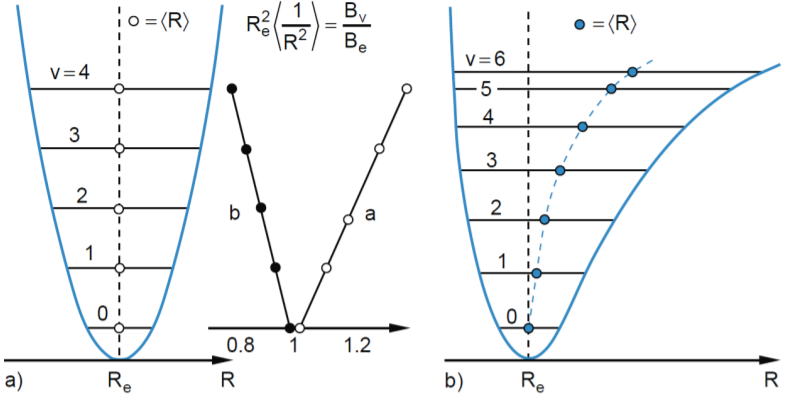
\includegraphics[width=.8\textwidth]{Q20/images/AfstandMellemEnerginiveauerneIToForskelligePotentialleApproksimationer.PNG}
    \caption{harmonisk oscillator-poteintiale sammenlignet med Morsepotentialet. Det kan ses, at afstanden mellem de vibrationelle tilstande er ens for den harmoniske oscillator, men bliver tættere og tættere end i Morsepotentialet.}
    \label{fig:Q20_AfstandMellemEnerginiveauer}
\end{figure}


\paragraph{Sammenhæng af vibration og rotation:} I virkeligheden er verden dog ikke så sort/hvid, at molekyler enten roterer eller vibrerer; de gør selvfølgelig begge dele, og deres bevægelse vil komme til at blive beskrevet som på \cref{fig:Q20_VibratingRotor}. Siden den totale energi af molekylet $E = E_\text{rot} 0 E_\text{vib} + E_\text{pot}$ skal være konstant ($\Dot{E} = 0$) må der findes en periodisk relation for ombytningen af vibrationenl energi, rotationel energi og potentiel energi. Dog er det meget besværligere at løse for et sådan system, og dette kan kun gøre ved brud af mange approksimationer og udviklinger (eng. expansions).

\begin{figure}[!h]
    \centering
    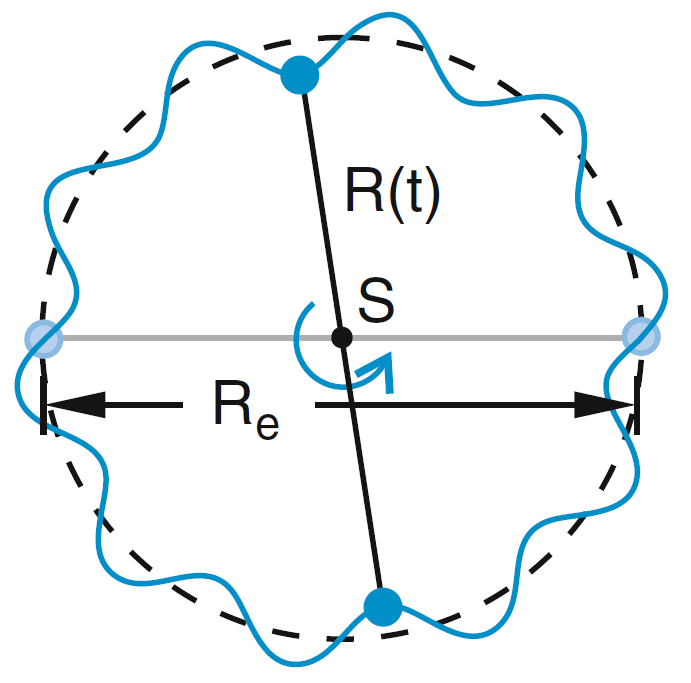
\includegraphics[width=.35\textwidth]{Q20/images/VibratingRotor.PNG}
    \caption{Vibrerende rotor.}
    \label{fig:Q20_VibratingRotor}
\end{figure}

På \cref{fig:Q20_VibratingRotor} kan det ses, at den vibrationelle frekvens er større end den rotationelle frekvens med én eller to størrelsesordener; molekylet vibrerer altså typisk 5-100 gange under én rotation. Dog, hvis man kigger på det, så vil hver vibrationelle tilstand have mange mulige rotationer tilknyttet, hvilket kan ses på \cref{fig:Q20_VibrationOgRotationPotential}.

\begin{figure}[!h]
    \centering
    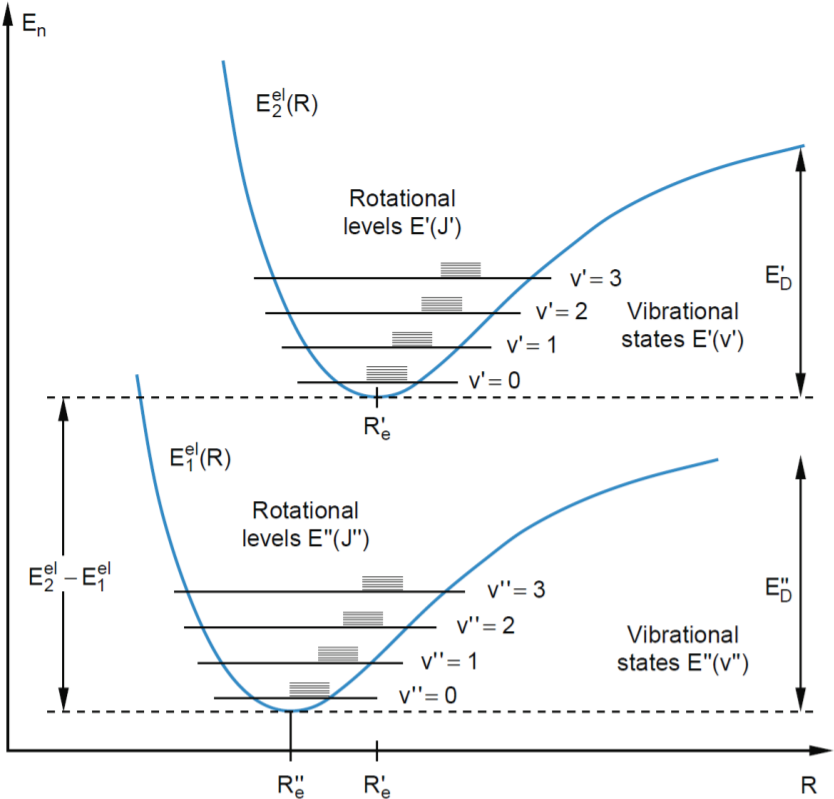
\includegraphics[width=.8\textwidth]{Q20/images/VibrationOgRotationIPotentialDiatomartMolekyle.PNG}
    \caption{Rotationelle og vibrationelle tilstande for et diatomart molekyle i to forskellige elektrontilstande.}
    \label{fig:Q20_VibrationOgRotationPotential}
\end{figure}